\onehalfspacing
\section{Đề số 34}

\begin{bt} 
	\hfill
	\begin{enumerate}[a.]
		\item Chứng minh: $5^{2014}-5^{2013}+5^{2012}$ chia hết cho 105 .
		\item Tìm số nguyên tố $\mathrm{p}$ sao cho $\mathrm{p}+2$ và $\mathrm{p}+4$ đều là số nguyên tố.
	\end{enumerate}
	\loigiai{
		\begin{enumerate}
			\item $5^{2014}-5^{2013}+5^{2012}=5^{2011}\left(5^3-5^2+5\right)$
			$=5^{2011}(125-25+5)=5^{2011} .105$ chia hết cho 105
			\item *) Nếu $\mathrm{p}=3 \mathrm{k}+1$ ta có: $2 \mathrm{p}+1=2(3 \mathrm{k}+1)+1=6 \mathrm{k}+3=3(2 \mathrm{k}+1)$ là hợp số ( trái gt)\\[5px]
			*) Nếu $\mathrm{p}=3 \mathrm{k}+2$ ta có $2 \mathrm{p}+4=2(3 \mathrm{k}+2)+2=6(\mathrm{k}+1)$ là hợp số ( trái $\mathrm{gt})$\\[5px]
			Vậy $p=3 k$, mặt khác $p$ là số nguyên tố nên $p=3$
		\end{enumerate}
	} 
\end{bt}

\begin{bt}
	Tìm x biết:
	\begin{enumerate}[a.]
		\item $|3-2 x|=x+1$
		\item $\left(\frac{1}{2}+\frac{1}{3}+\ldots+\frac{1}{2014}\right) \cdot x=\frac{2013}{1}+\frac{2012}{2}+\ldots+\frac{2}{2012}+\frac{1}{2013}$
	\end{enumerate}
	\loigiai{
		\begin{enumerate}
			\item Nếu $x \geq \frac{3}{2}$ thì $|3-2 x|=x+1 \Leftrightarrow 2 \mathrm{x}-3=\mathrm{x}+1 \Leftrightarrow \mathrm{x}=4$\\[5px] 
			Nếu $x<\frac{3}{2}$ thì $|3-2 x|=x+1 \Leftrightarrow 3-2 \mathrm{x}=\mathrm{x}+1 \Leftrightarrow 3 \mathrm{x}=2 \Leftrightarrow \mathrm{x}=\frac{2}{3}\\[5px]
			\text {Vậy } x=4 \text { hoặc } x=\frac{2}{3}$
			\item $\left(\frac{1}{2}+\frac{1}{3}+\ldots+\frac{1}{2014}\right) \cdot x=\frac{2013}{1}+\frac{2012}{2}+\ldots+\frac{2}{2012}+\frac{1}{2013} \\[5px]
			\Leftrightarrow\left(\frac{1}{2}+\frac{1}{3}+\ldots+\frac{1}{2014}\right) x=\frac{2012}{2}+1+\frac{2011}{3}+1 \ldots+\frac{2}{2012}+1+\frac{1}{2013}+1+1 \\[5px]
			\Leftrightarrow\left(\frac{1}{2}+\frac{1}{3}+\ldots+\frac{1}{2014}\right) x=\frac{2014}{2}+\frac{2014}{3}+\ldots+\frac{2014}{2012}+\frac{2014}{2013}+\frac{2014}{2014} \\[5px]
			\Leftrightarrow\left(\frac{1}{2}+\frac{1}{3}+\ldots+\frac{1}{2014}\right) x=2014\left(\frac{1}{2}+\frac{1}{3} \ldots+\frac{1}{2012}+\frac{1}{2013}+\frac{1}{2014}\right) \Leftrightarrow \mathrm{x}=2014$
		\end{enumerate}
	} 
\end{bt}

\begin{bt}
	\hfill 
	\begin{enumerate}[a.]
		\item Tìm $x ; y ; z$ biết $\frac{x}{y}=\frac{3}{2} ; 5 x=7 z$ và $x-2 y+z=32$.
		\item Cho $\frac{7 x+5 y}{3 x-7 y}=\frac{7 z+5 t}{3 z-7 t}$. Chứng minh: $\frac{x}{y}=\frac{z}{t}$.
		\item Tìm giá trị nhỏ nhất của $\mathrm{A}=|x-2013|+|2014-x|+|x-2015|$.
	\end{enumerate}
	\loigiai{
		\begin{enumerate}
			\item Ta có $\frac{x}{y}=\frac{3}{2} \Leftrightarrow \frac{x}{3}=\frac{y}{2} \Leftrightarrow \frac{x}{21}=\frac{y}{14}(1) ; 5 x=7 z \Leftrightarrow \frac{x}{7}=\frac{z}{5} \Leftrightarrow \frac{x}{21}=\frac{z}{15}$ (2)\\[5px]
			Từ (1) và (2) ta có: $\frac{x}{21}=\frac{y}{14}=\frac{z}{15}=\frac{x-2 y+z}{21-28+15}=\frac{32}{8}=4$\\[5px]
			Tìm được: $\mathrm{x}=84 ; \mathrm{y}=56 ; \mathrm{z}=60$
			\item Đặt: $\frac{7 x+5 y}{3 x-7 y}=\frac{7 z+5 t}{3 z-7 t}=\mathrm{k} \Rightarrow 7 \mathrm{x}+5 \mathrm{y}=\mathrm{k}(3 \mathrm{x}-7 \mathrm{y}) \Rightarrow(3 \mathrm{k}-7) \mathrm{x}=(7 \mathrm{k}+5) \mathrm{y} \Rightarrow \frac{x}{y}=\frac{7 k+5}{3 k-7}$\\[5px]
			Tương tự: $7 \mathrm{z}+5 \mathrm{t}=\mathrm{k}(3 \mathrm{z}-7 \mathrm{t}) \Rightarrow(3 \mathrm{k}-7) \mathrm{z}=(7 \mathrm{k}+5) \mathrm{t}\\[5px] 
			\Rightarrow \frac{z}{t}=\frac{7 k+5}{3 k-7}(2)$ (1)\\[5px]
			Từ (1) và (2) suy ra điều phải chứng minh.
			\item $\mathrm{A}=|x-2013|+|2014-x|+|x-2015|=(|x-2013|+|2015-x|)+|x-2014|$\\[5px]
			Ta có: $|x-2013|+|2015-x| \geq|x-2013+2015-x|=2$.\\[5px] Dấu " $=$ " xảy ra khi: $2013 \leq x \leq 2015(1)$\\[5px]
			Lại có: $|x-2014| \geq 0$. Dấu "=" xảy ra khi $x=2014$ (2).\\[5px] 
			Từ (1) và (2) Ta có minA = 2. Dấu "=" xảy ra
			khi $x=2014$
		\end{enumerate}
	} 
\end{bt}

\begin{bt}
	Cho tam giác $A B C$ cân $(A B=A C)$. Trên cạnh $B C$ lấy điểm $D$ trên tia đối tia $C B$ lấy điểm $E$ sao cho $\mathrm{BD}=\mathrm{CE}$. Các đường thẳng vuông góc với $\mathrm{BC}$ kẻ từ $\mathrm{D}$ và $\mathrm{E}$ cắt $\mathrm{AB}$ và $\mathrm{AC}$ lân lượt ở $\mathrm{M}$ và N. Gọi I là giao điểm của $\mathrm{MN}$ và $\mathrm{BE}$.
	\begin{enumerate}[a.]
		\item Biết $\mathrm{AB}<\mathrm{BC}$. Chứng minh: $\hat{\mathrm{A}}>60^{\circ}$.
		\item Chứng $\operatorname{minh} \mathrm{IM}=\mathrm{IN}$
		\item Chứng minh đường thẳng vuông góc với $\mathrm{MN}$ tại I luôn đi qua 1 điểm cố định khi $\mathrm{D}$ thay đối trên cạnh $B C$.
	\end{enumerate}
	\loigiai{
		$$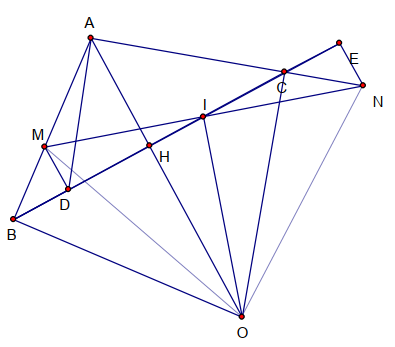
\includegraphics[width=0.5\textwidth]{34-4-lg.png}$$
		\begin{enumerate}
			\item Do $\mathrm{AB}<\mathrm{BC}$ nên $A>B$. mà $B=C$ vì tam giác $\mathrm{ABC}$ cân Mà $A+B+C=180^{\circ}$ nên ta có $A>60^{\circ}$ (HS có thể $c / \mathrm{m}$ bằng phản chứng)
			\item HS chứng minh được $\Delta \mathrm{BDM}=\Delta \mathrm{CEN}$ suy ra $\mathrm{EN}=\mathrm{DM}$ HS chứng minh được $\triangle \mathrm{IDM}=\Delta \mathrm{IEN}$ suy ra $\mathrm{IN}=\mathrm{IM}$
			\item Kẻ $\mathrm{AH}$ vuông góc với $\mathrm{BC}$. Gọi $\mathrm{O}$ là giao điểm của $\mathrm{AH}$ và đường thẳng vông góc với $\mathrm{MN}$ ở $\mathrm{I}$.\\[5px] 
			HS chứng minh được $\mathrm{O}$ là điểm cố định.
		\end{enumerate}
	}
\end{bt}